\section{Testing}
\subsection{Microservices}
\subsubsection{Tests of a single microservices}
For managing the tests, in general, during the development, once a feature was ready it was tested. 
The procedure described in the Design document was followed; however, due to the fact that many spring
components and classes do already many things, unit tests of single class sometimes didn't make much 
sense, because it would have been necessary to mock many Spring features, that are supposed to be already
tested and working properly. \\
For the projects, the process of testing usually followed this life cycle: repositories have been tested firsts, then the services, that cover
the business functions of the project under consideration, and then the controllers, for which two kinds of tests were performed: a unit and
an integration test.
These integration tests involves all the stacks that were developed in the projects: indeed, from here, the connection to the APIs with HTTP/
HTTPS requests are tested: this methods usually call the business functions, that modifies the databases by means of repositories.
If error occurs, the classes in the advice packages come into help, and, therefore, they are tested as well. \\
For what concerns the tests that regards interfaces that allows to share events with other microservices, as soon as it was possible to have
them working they were tested as well. 
However, it is worth to note that the real integration between microservices have been tested with JMeter. This is because TODO TANG. \\
The same things holds for the test of the service registry and for the forwarding of requests to other microservices by means of the Zuul
gateway.  \\
The approach taken for all the tests mentioned above (the ones with JMeter excluded), is white box testing. 
Here it follows a brief report on the coverage, with some comments. The images are taken
from the report generated by JaCoCo. \\

\par 
First of all the coverage of the API gateway is shown.

\begin{figure}[H]
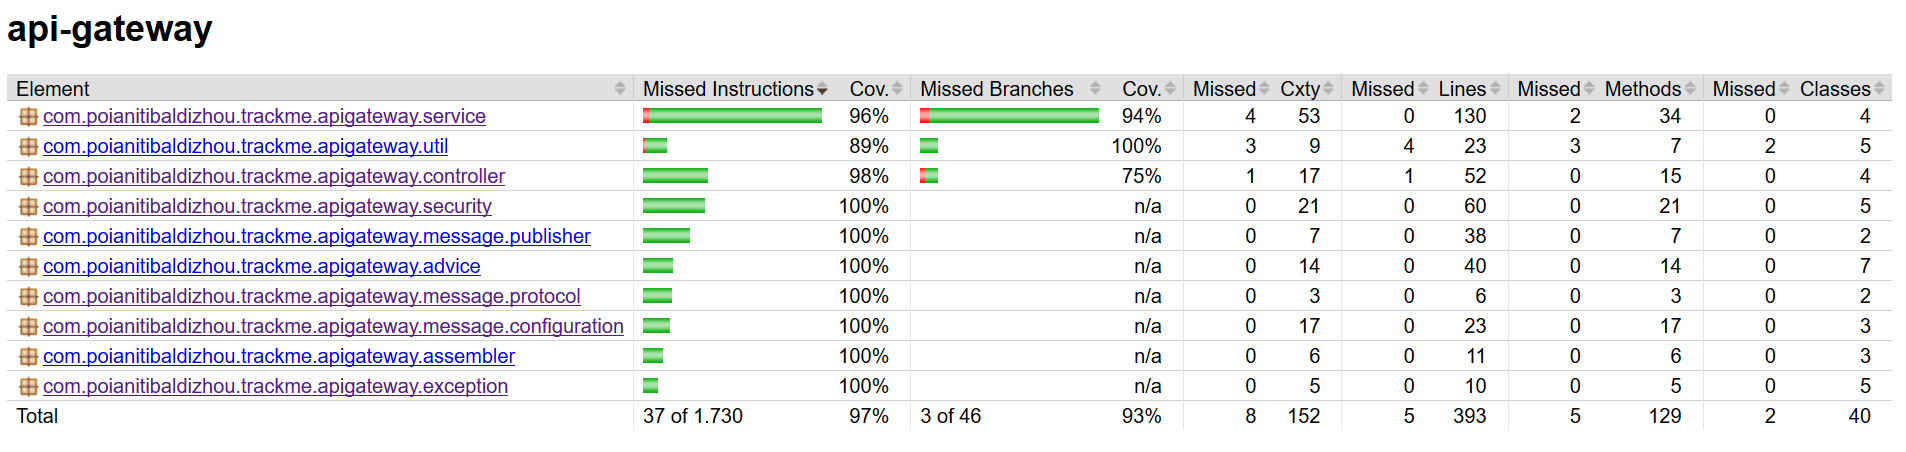
\includegraphics[width=\linewidth]{images/CoverageApigateway.png}
\caption{ API gateway coverage}
\label{fig:cvgapigateway}
\end{figure}


As one may notice, the entity and the filter packages are not present. Indeed, filters have been tested with JMeter, and therefore are not
present here. 
Furthermore, entity classes are basically only attributes and methods that are not shown since they are auto generated with lombok. \\
Finally, all the other lombok auto generated methods have been excluded from the coverage.

\par 
Similar reasoning applies also to the coverage of the individual request service.
\begin{figure}[H]
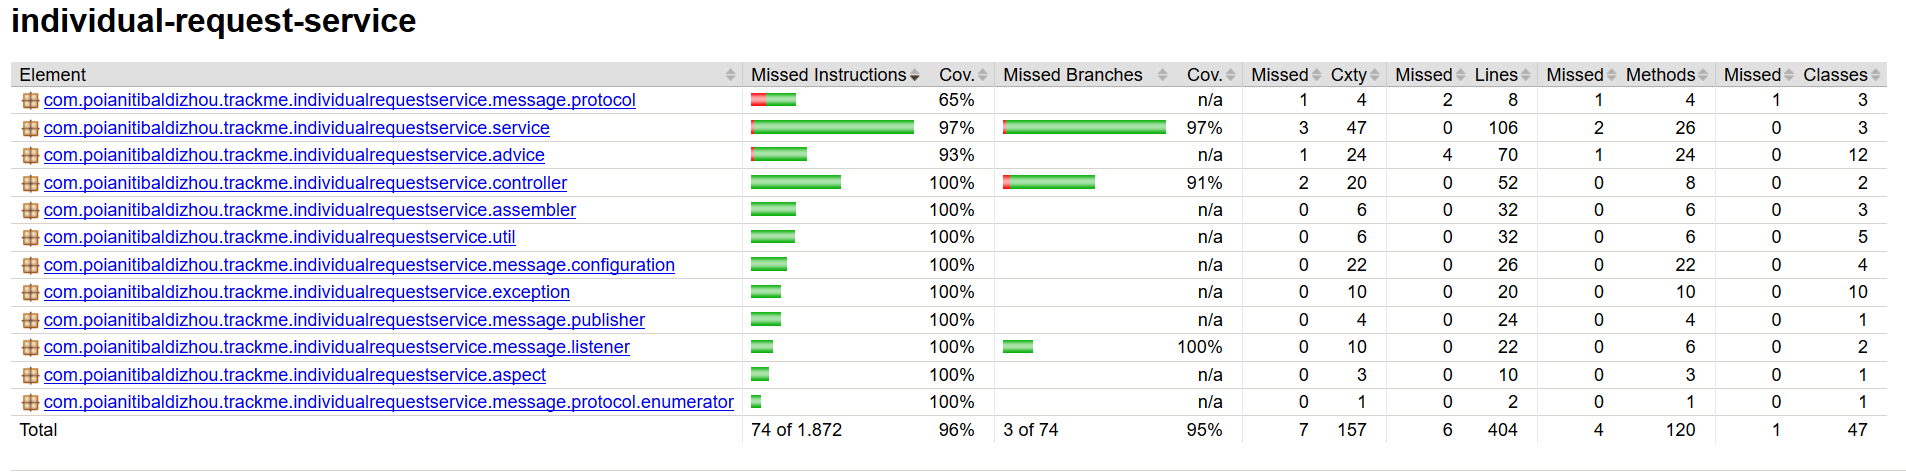
\includegraphics[width=\linewidth]{images/CoverageIndividualrequestservice.png}
\caption{ Individual request service coverage}
\label{fig:cvgindividual}
\end{figure}

\par 
Same things hold also for the group request service.
\begin{figure}[H]
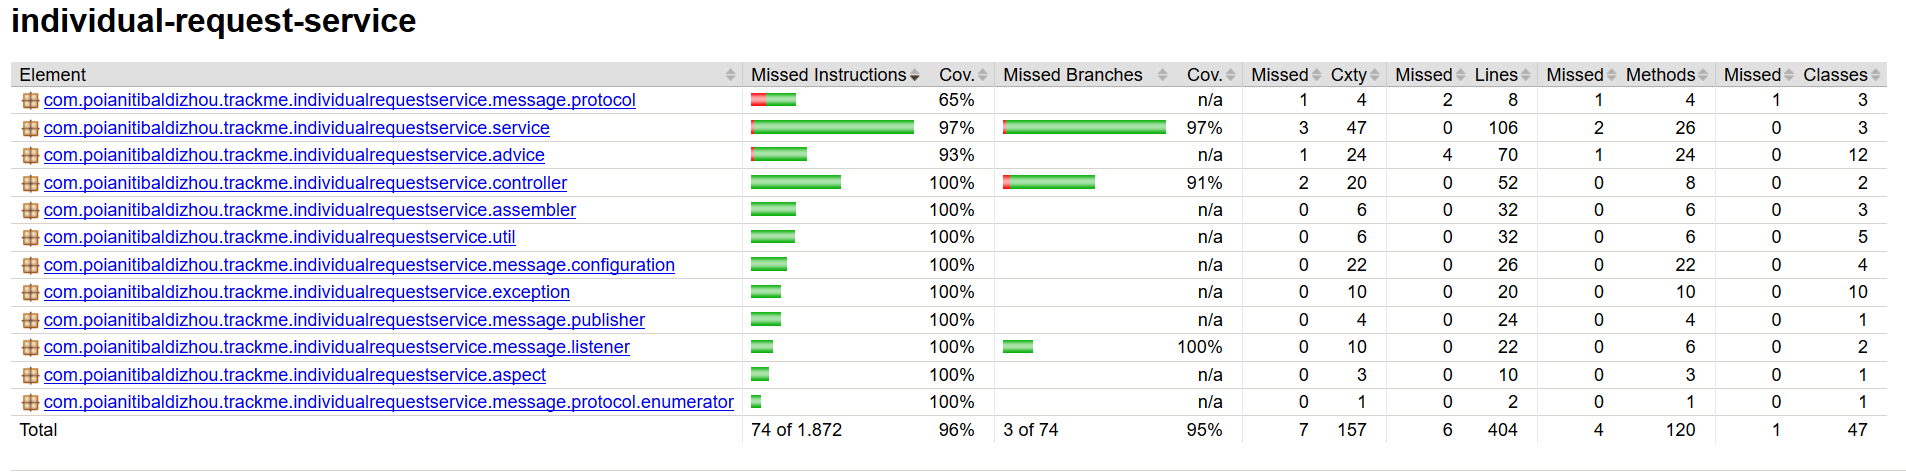
\includegraphics[width=\linewidth]{images/CoverageIndividualrequestservice.png}
\caption{ Group request individual service coverage}
\label{fig:cvggroup}
\end{figure}

\par
For what concerns the share data service, here follows the image of the coverage. The same comments
are valid also in this situation.

\begin{figure}[H]
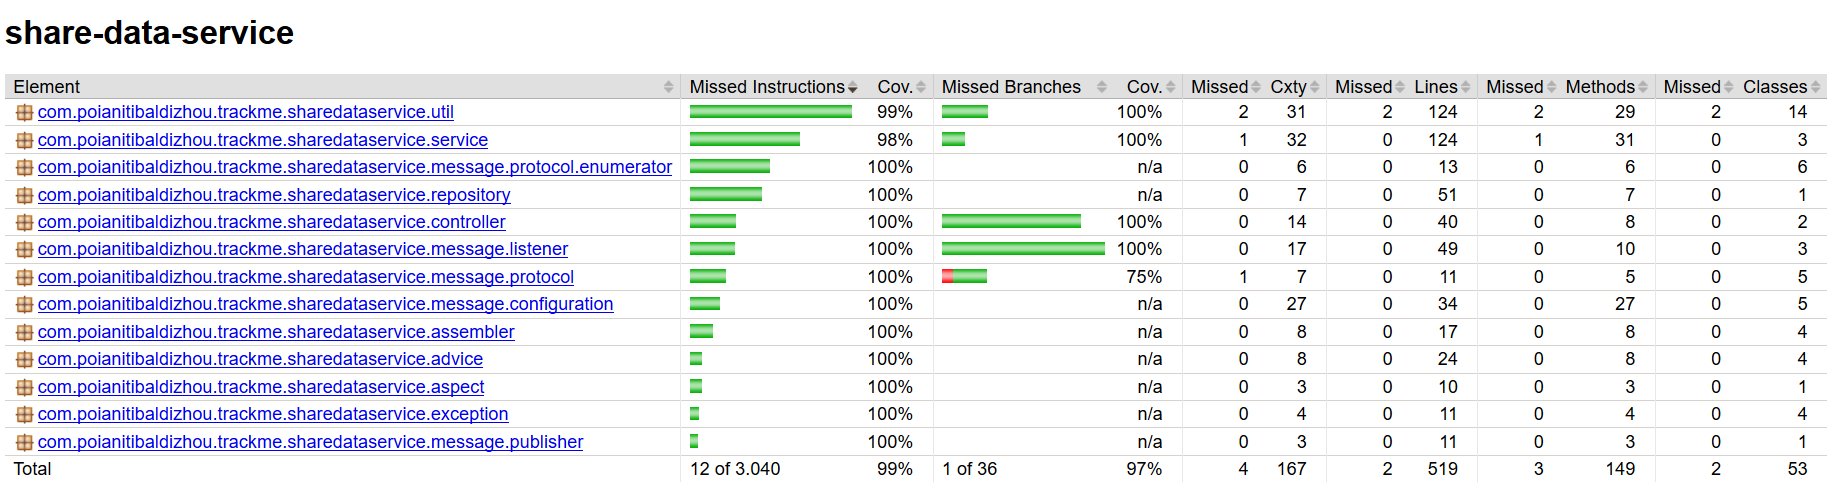
\includegraphics[width=\linewidth]{images/CoverageSharedataservice.png}
\caption{ Share data service coverage}
\label{fig:cvgshare}
\end{figure}


\subsubsection{JMeter} 
// TODO TANG TANG


\subsection{Android application}
// TODO TANG TANG AND MATTIA 
